\chapter{Artigo 01: DCCA multi cross-correlation analysis applied on EEG signals to study motor
activity (Real/Imaginary)}
\label{cap:paper_01}

\begin{flushright}
    ``That brain of mine \\
    is something more\\
    than merely mortal,\\
    as time will show.''\\[10px]
    (Ada Lovelace)
\end{flushright}

O primeiro artigo apresentado, \emph{DCCA multi cross-correlation analysis applied on EEG signals to study motor activity (Real/Imaginary)}~\cite{RIBEIRO2025107419}, narra uma pesquisa utilizando o \dmc~na busca de padrões cerebrais, através do estudo das séries temporais oriundas de um experimento (de movimentos reais e imaginários dos membros do corpo) monitorado pelas gravações das ondas do cérebro por um aparelho de eletroencefalograma. O artigo trabalha com o \pdcca com a mesma fonte de dados que o artigo intitulado \emph{Statistical study of the EEG in motor tasks (real and imaginary)}~\cite{Oliveira2023}, utilizando o \pdcca~apresentado no Anexo~\ref{an:a}, e representa um avanço técnico em relação ao anterior.

\begin{figure}[!htb]
	\centering
	\caption{Desvio padrão dos valores do \dmc para cada uma das tarefas}
	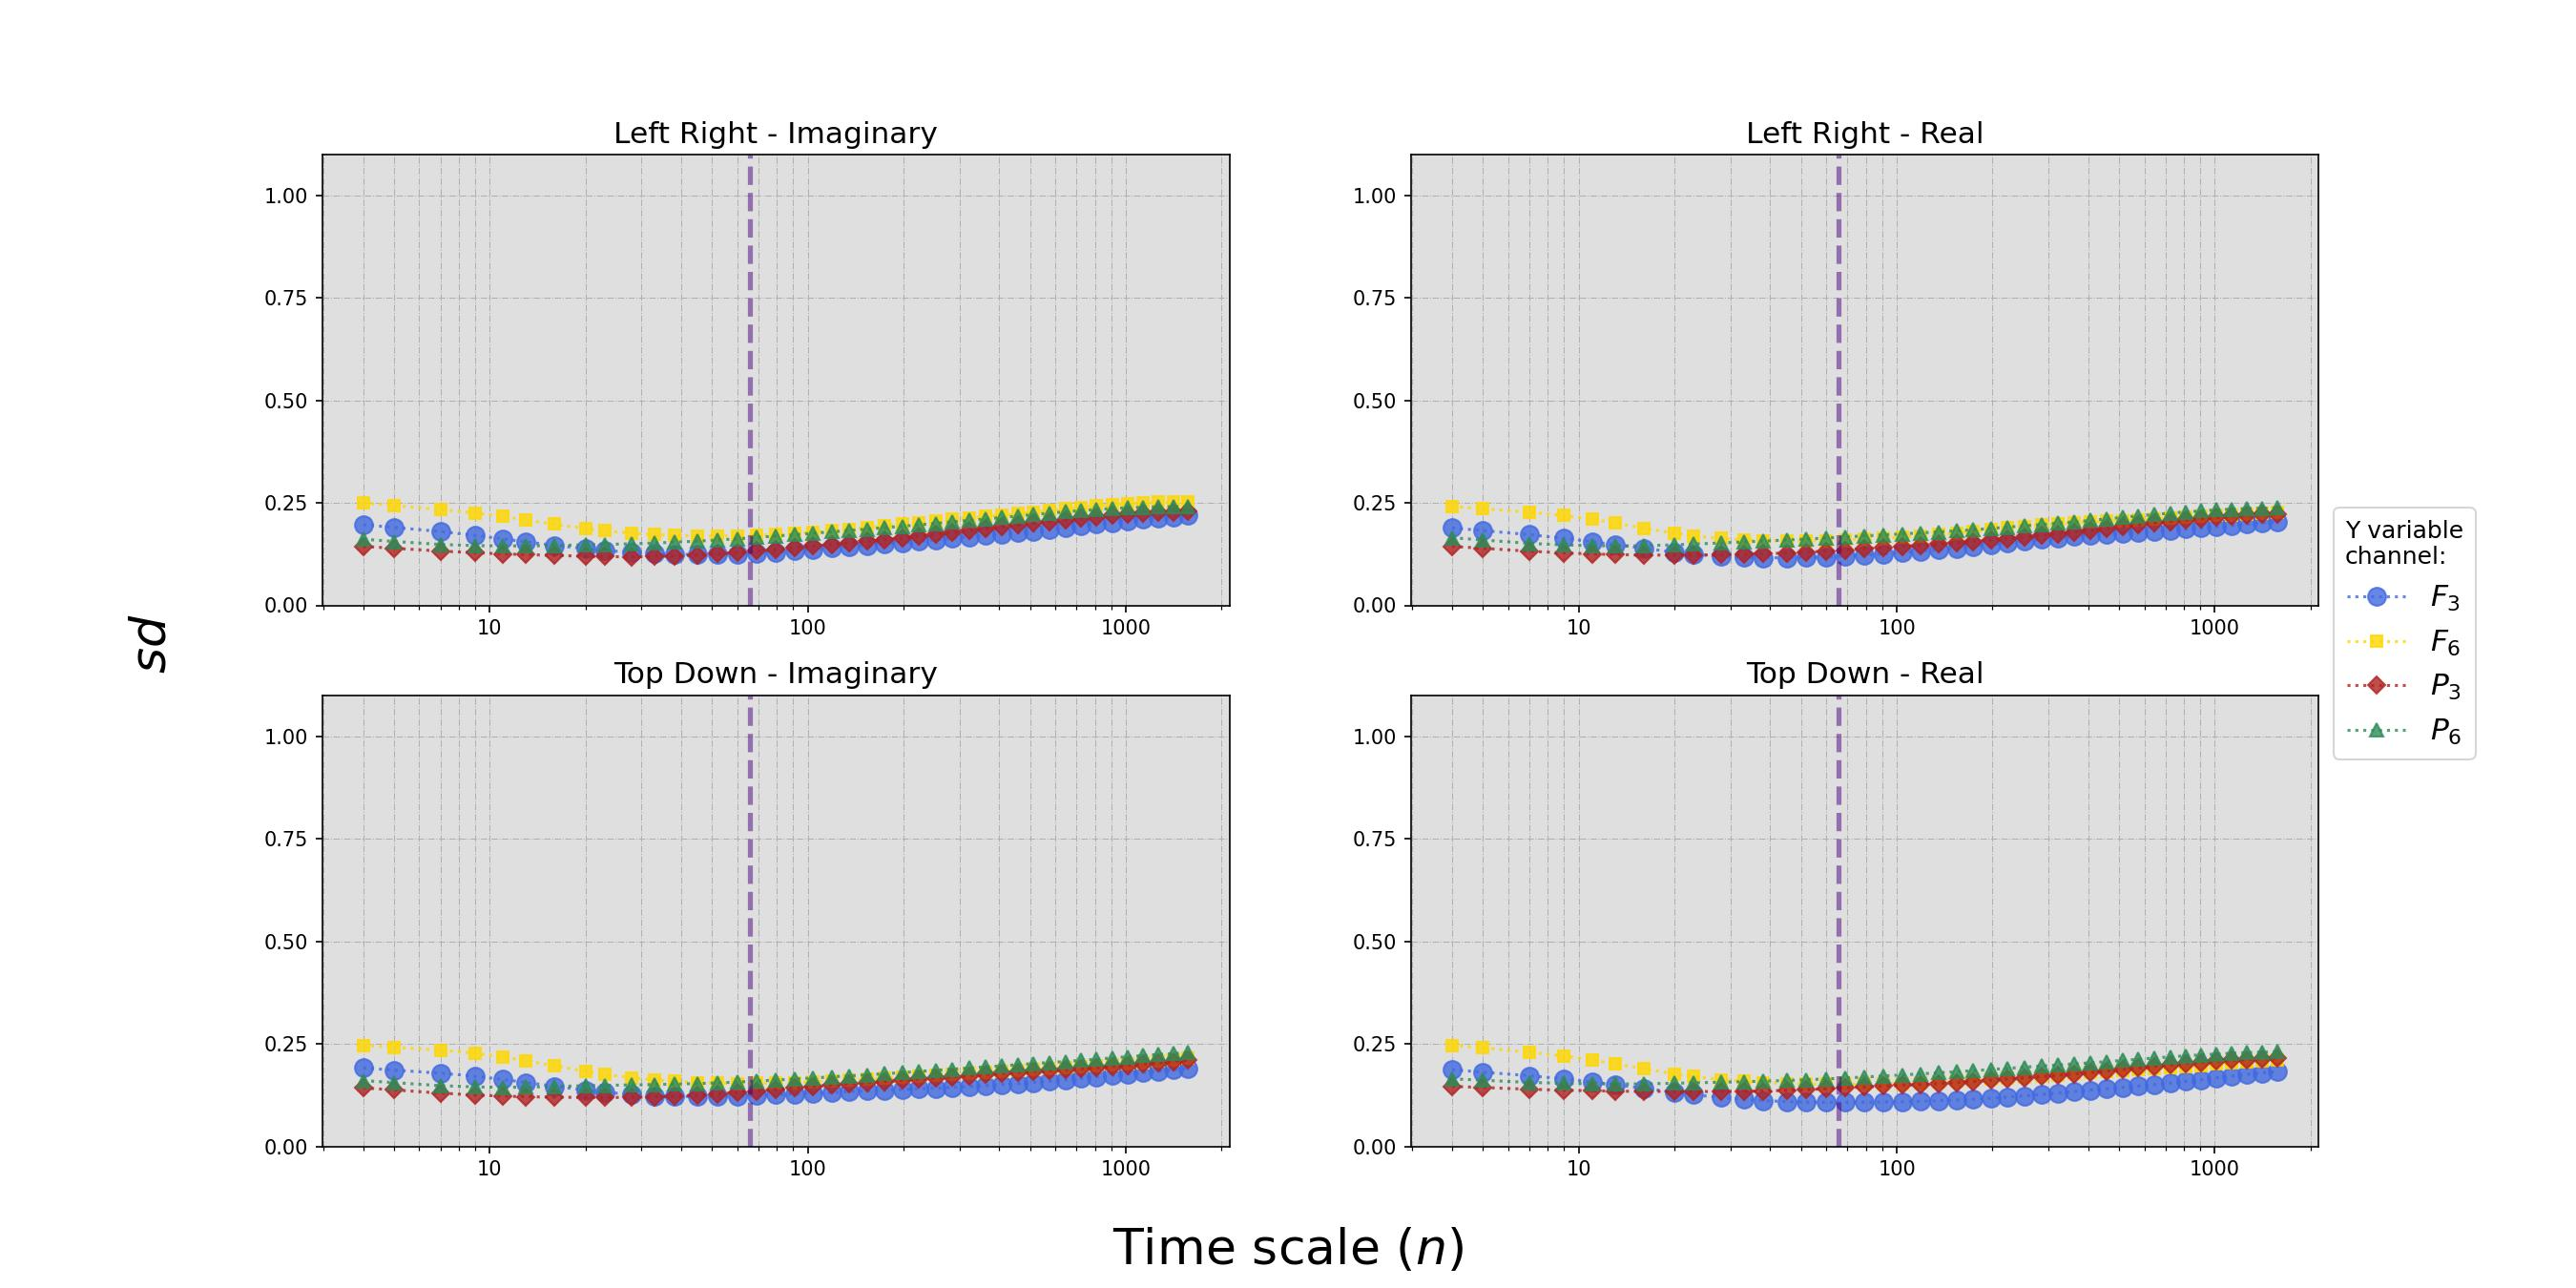
\includegraphics[width=.8\textwidth]{./Figures/art_01/std pop.jpg}
	\\{\footnotesize Fonte: Elaborada pelos autores}
	\label{fig:a01_sd}
\end{figure}

No Artigo de 2023, apenas um subconjunto de 11 indivíduos de universo de 109. Já no artigo de 2025, 108 dos 109 indivíduos foram analisados. Encarando o dilema de, trabalhar com um ambiente de mais alto nível, capaz de manipular o conjunto de dados e visualizar os resultados de foma mais prática e automatizada, com sacrifício do desempenho, ou trabalhar em baixo nível, como maior velocidade de cálculos e menor praticidade para trabalhar, uma solução intermediária foi adotada: os dados foram baixados, carregados, editados e preparados utilizando um ambiante Python, os cálculos foram feitos através de um programa escrito em C e a visualização dos resultados novamente em Python. As chamadas do programa em C foram feitas dentro do código Python, utilizando a biblioteca \emph{subprocess}.

\begin{figure}[!htb]
	\centering
	\caption{Médias dos valores do \dmc para cada uma das tarefas}
	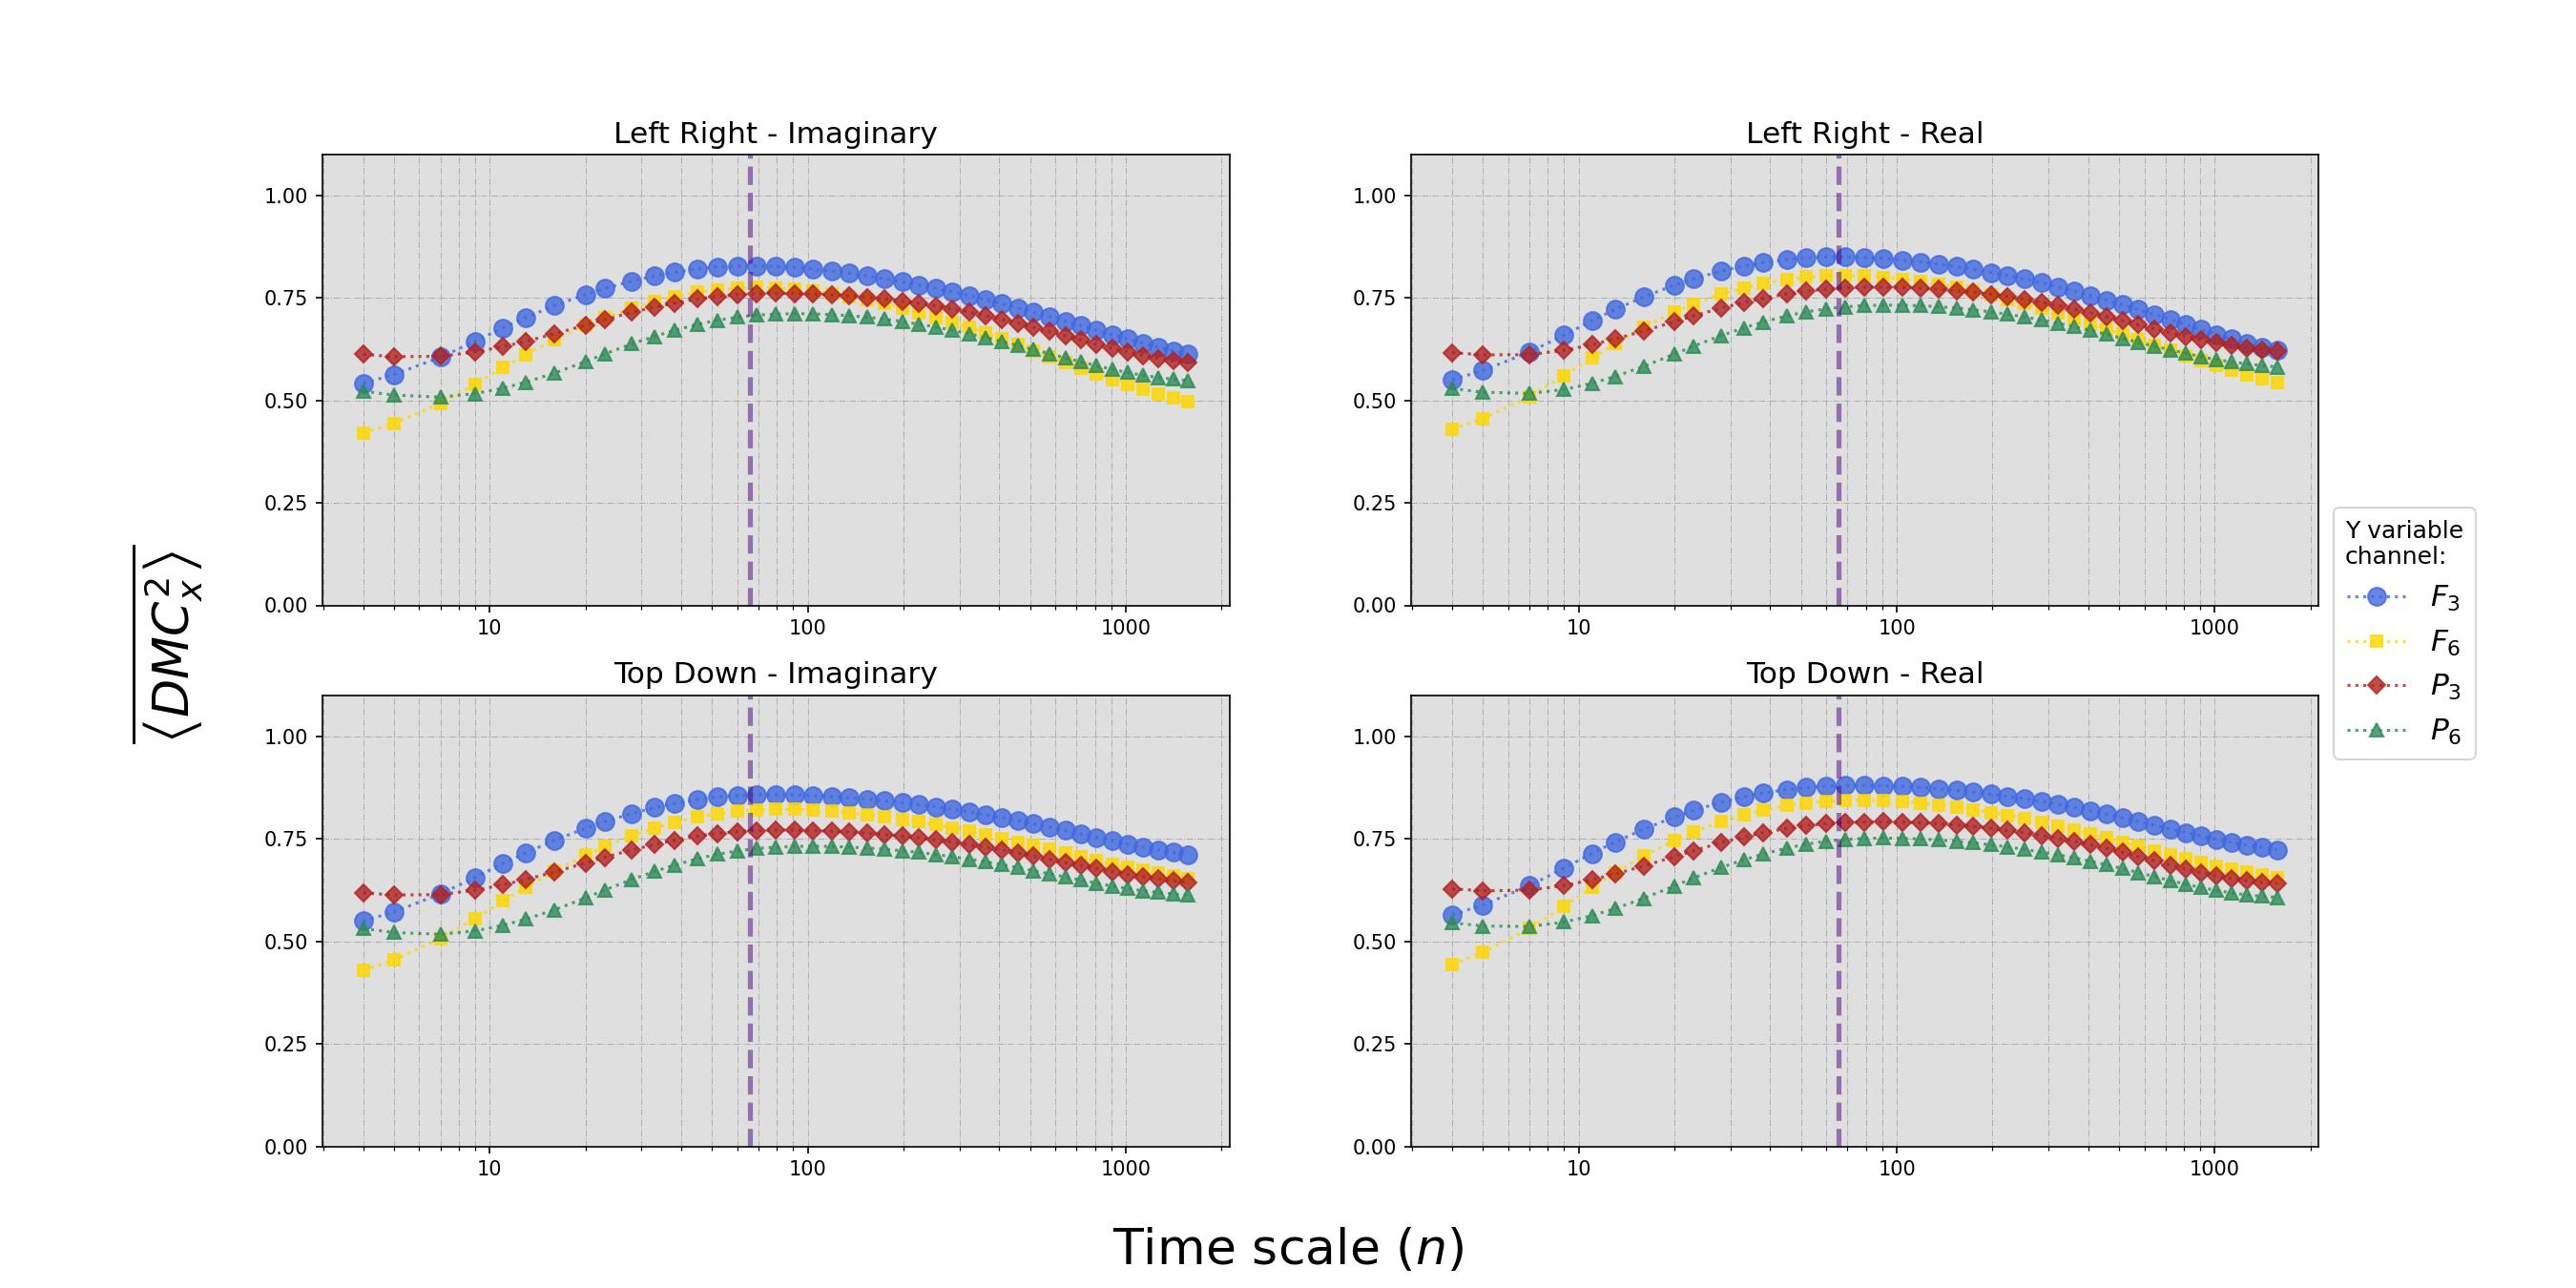
\includegraphics[width=.8\textwidth]{./Figures/art_01/mean.jpg}
	\\{\footnotesize Fonte: Elaborada pelos autores}
	\label{fig:a01_mean}
\end{figure}

A implementação em C executa a inversão da matriz $\rho^{-1}(n)$, apresentada na Equação~\ref{eq:p_dcca_matrix} em codificação direta, como mostrado na Equação~\ref{eq:dmc_3x_y}. Significando que, para cada quantidade de variáveis independentes que se queira estudar, um novo programa deve ser escrito.

\begin{equation}
    \begin{split}
    DMC_{x}^{2} \quad = \quad & \Big( \Big. \rho^{2}_{X_{2},X_{3}} \times \rho^{2}_{Y,X_{1}}- \rho^{2}_{Y,X_{1}} + \rho^{2}_{X_{1},X_{3}}\times \rho^{2}_{Y,X_{2}}-\rho^{2}_{Y,X_{2}} \\
    &+ 2 \times \rho_{X_{1},X_{2}} \times \rho_{Y,X_{1}} \times \rho_{Y,X_{2}}   - 2 \times \rho_{X_{1},X_{3}} \times \rho_{X_{2},X_{3}} \times \rho_{Y,X_{1}} \\
    &+ \rho^{2}_{X_{1},X_{2}} \times \rho^{2}_{Y,X_{3}}-\rho^{2}_{Y,X_{3}} + 2 \times \rho_{X_{1},X_{3}} \times \rho_{Y,X_{1}} \times \rho_{Y,X_{3}} \\ 
    &- 2 \times \rho_{X_{1},X_{2}} \times \rho_{X_{2},X_{3}} \times \rho_{Y,X_{1}} \times \rho_{Y,X_{3}} \\
    &- 2 \times \rho_{X_{1},X_{2}} \times \rho_{X_{1},X_{3}} \times \rho_{Y,X_{2}} \times \rho_{Y,X_{3}} \\
    &+ 2 \times \rho_{X_{2},X_{3}} \times \rho_{Y,X_{2}} \times \rho_{Y,X_{3}} \Big. \Big)    \quad \Big/ \\
    & \Big( \Big. \rho^{2}_{X_{1},X_{2}} + \rho^{2}_{X_{1},X_{3}} + \rho^{2}_{X_{2},X_{3}} - 2 \times \rho_{X_{1},X_{2}} \times \rho_{X_{1},X_{3}} \times \rho_{X_{2},X_{3}}^{-1}\Big. \Big)  \\
    \end{split}
    \label{eq:dmc_3x_y} 
    \end{equation}

A pesquisa utilizou-se exaustivamente da análise de gráficos para chegar nas conclusões revisadas pelos pares. A quantidade de figuras excederia o tamanho do artigo, forçando a criação de um repositório \emph{online} no endereço abaixo:

\begin{center}
	\url{https://255ribeiro.github.io/Multi_Cross-correlation_EEG/}
\end{center}

\begin{figure}[!htb]
	\centering
	\caption{Mediana dos valores do \dmc para cada uma das tarefas}
	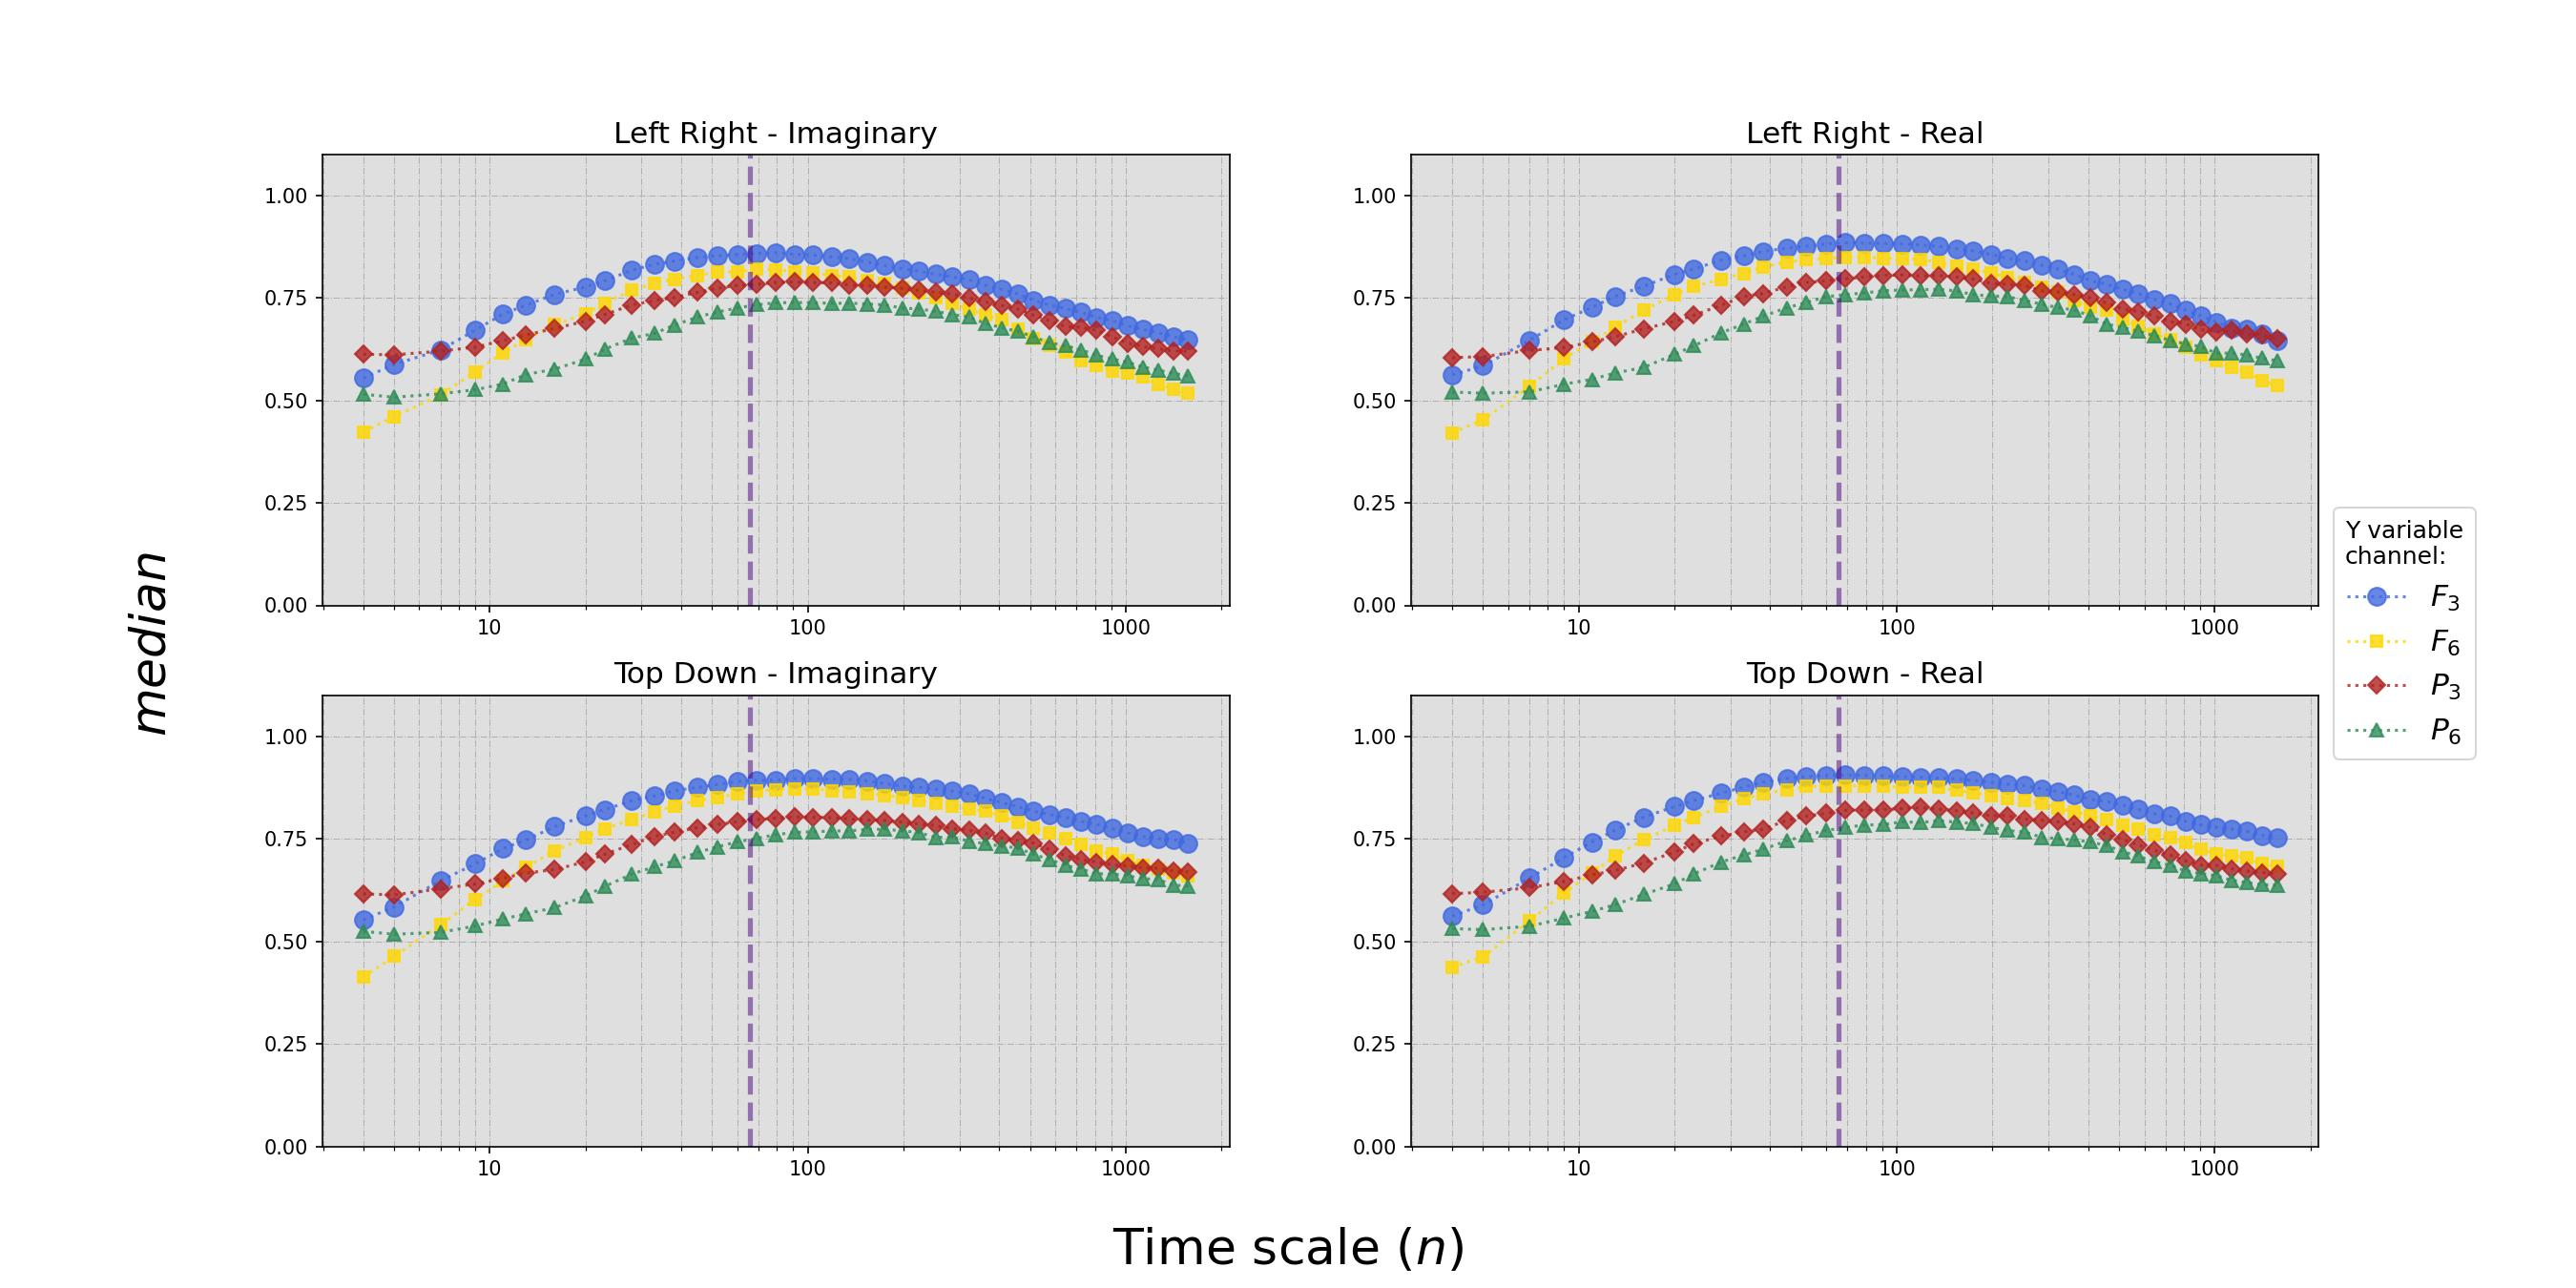
\includegraphics[width=.8\textwidth]{./Figures/art_01/median.jpg}
	\\{\footnotesize Fonte: Elaborada pelos autores}
	\label{fig:a01_median}
\end{figure}

As Figuras~\ref{fig:a01_sd},~\ref{fig:a01_mean}~e~\ref{fig:a01_median} mostram grande consistência entre a população, no entanto é possível observar características nos gráficos de cada indivíduo que apontam para uma assinatura individual, como uma impressão digital, como explicado no artigo. Para facilitar o entendimento das análises, alguns vídeos que apresentam sequencialmente os resultados das tarefas de cada individuo foram criados e colocados no repositório \emph{online}.

Nos termos da quantidade de dados analisados, a implementação carece de melhorias e otimizações. Passar os dados para C através da biblioteca \emph{subprocess} é um processo trabalhoso, exigindo a gravação dos arquivos tratados em arquivos formatados conforme as regras estabelecidas no código em C. generalizações do algorítimo para um número qualquer de séries temporais e do cálculo da inversão da matriz também devem ser implementados para expandir as possibilidades em trabalhos futuros.









\includepdf[pages=-, pagecommand={\thispagestyle{plain}}]{./Papers_publi/Ribeiro_2025_DCCA_multi_cross-correlation_analysis_applied_on_E.pdf}
